\documentclass[12 pt]{book} 

\usepackage{amsmath, amsthm, amssymb, mathrsfs}
\usepackage{graphicx}
\usepackage{cite}
\usepackage[left=3.0cm,top=3.0cm,right=3.0cm,nohead,foot=3.0cm]{geometry}
\usepackage{fancyhdr}

\bibliographystyle{ieeetr} 

\pagestyle{empty}
\renewcommand{\v}[1]{\ensuremath{\mathbf{#1}}} % for vectors
\newcommand{\gv}[1]{\ensuremath{\mbox{\boldmath$ #1 $}}} 
% for vectors of Greek letters
\newcommand{\uv}[1]{\ensuremath{\mathbf{\hat{#1}}}} % for unit vector
\newcommand{\abs}[1]{\left| #1 \right|} % for absolute value
\newcommand{\avg}[1]{\left< #1 \right>} % for average
\let\underdot=\d % rename builtin command \d{} to \underdot{}
\renewcommand{\d}[2]{\frac{d #1}{d #2}} % for derivatives
\newcommand{\dd}[2]{\frac{d^2 #1}{d #2^2}} % for double derivatives
\newcommand{\pd}[2]{\frac{\partial #1}{\partial #2}} 
% for partial derivatives
\newcommand{\pdd}[2]{\frac{\partial^2 #1}{\partial #2^2}} 
% for double partial derivatives
\newcommand{\pdc}[3]{\left( \frac{\partial #1}{\partial #2}
 \right)_{#3}} % for thermodynamic partial derivatives
\newcommand{\ket}[1]{\left| #1 \right>} % for Dirac bras
\newcommand{\bra}[1]{\left< #1 \right|} % for Dirac kets
\newcommand{\braket}[2]{\left< #1 \vphantom{#2} \right|
 \left. #2 \vphantom{#1} \right>} % for Dirac brackets
\newcommand{\matrixel}[3]{\left< #1 \vphantom{#2#3} \right|
 #2 \left| #3 \vphantom{#1#2} \right>} % for Dirac matrix elements
\newcommand{\grad}[1]{\gv{\nabla} #1} % for gradient
\let\divsymb=\div % rename builtin command \div to \divsymb
\renewcommand{\div}[1]{\gv{\nabla} \cdot #1} % for divergence
\newcommand{\curl}[1]{\gv{\nabla} \times #1} % for curl

% ABSTRACT

\newenvironment{abstract}
{\thispagestyle{empty}
\begin{center}
\vspace*{1.5cm}
{\Large \bfseries Abstract}
\end{center}
\vspace{0.5cm}
\begin{quote}}
{\end{quote}}

% DEDICATION
%
% The dedication environment makes sure the dedication gets its
% own page and is set out in verse format.

\newenvironment{dedication}
{\thispagestyle{empty}
  \begin{center}
  \vspace*{1.5cm}
  {\LARGE }
  \end{center}
  \vspace{0.5cm}
  \begin{verse}\begin{center}}
{\end{center}\end{verse}}


% ACKNOWLEDGEMENTS
%
% The acknowledgements environment puts a large, bold, centered 
% "Acknowledgements" label at the top of the page. The acknowledgements
% themselves appear in a quote environment, i.e. tabbed in at both sides, and
% on its own page.

\newenvironment{acknowledgements}
{\thispagestyle{empty}
\begin{center}
\vspace*{1.5cm}
{\Large \bfseries Acknowledgements}
\end{center}
\vspace{0.5cm}
\begin{quote}}
{\end{quote}}

\begin{document}
\title{Circuit QED with Highly Multimodal Photon-Qubit Strong Coupling}

\author{Alexander Pease \\
\texttt{apease@princeton.edu}\\
\\
Advisor: Andrew Houck\\
\\
A Thesis presented to the\\ 
Department of Physics of
Princeton University\\
in Candidacy for the Degree of \\
Bachelor of Arts\\
\\
\\}

\date{May 7th, 2012}
\maketitle

%%%%%%%%%%%%%%%%%
\begin{center}
This paper represents my own work in accordance with University regulations. \par
\vspace{1.5cm}
\hspace{0.5cm} \makebox[3.5in]{\hrulefill}\\
Alexander Pease
\end{center}

%%%%%%%%%%%%%%%%%
\newpage
\begin{abstract}
Text here
\end{abstract}

%%%%%%%%%%%%%%%%%
\newpage
\begin{acknowledgements}
Text here
\end{acknowledgements}



%: ----------------------- contents ------------------------

\setcounter{secnumdepth}{3} % organisational level that receives a numbers
\setcounter{tocdepth}{3}    % print table of contents for level 3
\tableofcontents            % print the table of contents
% levels are: 0 - chapter, 1 - section, 2 - subsection, 3 - subsection


%: ----------------------- list of figures/tables ------------------------

\listoffigures	% print list of figures

\listoftables  % print list of tables

%%%%%%%%%%%%%%%%%%%%%%%%%%%%%%%%%%%%%%%%%%%%%%%%%%%%%%%%%%%%%%%%%%%%%%%
%%%%%%%%%%%%%%%%%%%%%%%%%%%%%%%%%%%%%%%%%%%%%%%%%%%%%%%%%%%%%%%%%%%%%%%
%%%%%%%%%%%%%%%%%%%%%%%%%%%%%%%%%%%%%%%%%%%%%%%%%%%%%%%%%%%%%%%%%%%%%%%
%%%%%%%%%%%%%%%%%%%%%%%%%%%%%%%%%%%%%%%%%%%%%%%%%%%%%%%%%%%%%%%%%%%%%%%
%%%%%%%%%%%%%%%%%%%%%%%%%%%%%%%%%%%%%%%%%%%%%%%%%%%%%%%%%%%%%%%%%%%%%%%
\chapter{Introduction}\label{chap:Introduction}
%We live in a world of information. Information is the fuel driving every facet of our society; from our daily email exchanges to the global economy to the DNA of every living organism, we are comfortable in our understanding that information is of fundamental importance. We are perhaps most familiar with a mathematical definition of the ``bit"- a binary digit, zero or one, the basis of all logical computation. 

We live in a world of information. Information is the fuel driving every facet of our lives, from our daily email exchanges to the global economy to the DNA the makes us unique. And yet we tend to consider information in simplistic terms. The ``bit" - a binary digit, zero or one, the basis of all logical computation - is an absolute idea. Perceived as being the fundamental unit of information, John Wheeler once described Nature as ``it from bit."

This conception of information is fundamentally wrong, or at least incomplete. Since the rise of quantum mechanics at the beginning of the 20$^{\mathrm{th}}$ century, physicists have understood that we live in world of inherent randomness and non-locality. And so, as physicists are wont to do, Richard Feynman posed a difficult question: ``What is information in a quantum mechanical world?" 

The field of quantum computing not only seeks to answer this question but also to control quantum information for practical purposes. This has been motivated by theoretical work realizing the potential for quantum computers to outperform their digital counterparts, SHORE AND GROVER ALGORITHMS, quantum simulation. 

Research into quantum computing has utilized numerous viable architectures. This thesis is an investigation into one such implementation, circuit quantum electrodyanmics. The underlying science of this design draws upon existing literature on cavity quantum electrodynamics. This introduction will give a brief overview into both fields. 


%introduce other branches of quantum computing, then focus on cQED and it's origins in cavity QED
%\cite{LossDiVincenzo} first electron spin proposal



%Factor large numbers /cite{}, simulate quantum physics /cite{}. Shore and Grover’s algorithms.  RSA?
%Exponential parallel processing by quantum mechanics
%Compare to binary bits…n qubits can be in a superposition of 2^n basis states. Applying a single operation simultaneously computes output for all 2^n inputs. 
%Information is inherently a physical quantity, and the physics of information is the physics of all matter [Landauer1991]

\section{Cavity quantum electrodynamics}
Cavity quantum electrodynamics (cavity QED) is the study of the interaction between light and matter at the quantum level. Despite being wave-like in nature, electromagnetic fields are composed of discrete packets known as photons. This quantization, rather than being a matter of bookkeeping, has subtle and far reaching effects \cite{Schuster}. Amazingly, this wave-like behavior is not just an emergent phenomenon arising from millions of photonic constituents; even a single photon displays a wave-particle duality. 

The simplest CQED system places an atom inside a confined cavity. The walls of the cavity act as mirrors, such that when a photon is introduced it is reflected back and forth as many as one million times \cite{Vahala2003}. This reflection allows for the increased probability of the photonic and atomic systems coupling. As such, it is an excellent system by which to study the fundamental light-matter interactions. 

Yet, ignoring the atom for a moment, this system is also ideal for considering a very subtle question: ``What is the shape of a photon?" Both the spatial and temporal distributions of energy are not fixed, but are dependent and \emph{controllable} by the boundary conditions imposed upon the photon by matter \cite{Schuster}. By engineering a cavity, we can control the physical properties of quantized electromagnetic radiation. 

Coupled to an atomic system, a photon is no longer simply oscillating in the cavity. The two subsystems may interact, transferring energy, even destroying the photon (a non-conserved bosonic particle). The atom may be excited into a higher energy state, eventually decaying back down via spontaneous emission. Remarkably, the existence of the cavity also controls the behavior of the atom in this regard, suppressing the emission of any photons that do not ``fit" inside the cavity. Cavity QED allows one to suppress, enhance, and even make coherent the radiative decay of an atom, allowing one to study and engineer this mysterious quantum process \cite{Schuster}.

This coupling also affects the states of the cavity. Just as the atoms energy levels are affected, the existence of an atomic system shifts the possible states of the cavity! Considering the system as a whole, it is possible to infer quantum information about the atom simply by measuring the cavities properties. This will be discussed in detail in Chapter \ref{chap:Theoretical}. 

Such phenomena are just the tip of the iceberg. The quantum nature of such systems gives rise some truly spectacular behavior. This thesis will touch on a few, such as nonlinear Vacuum Rabi effects in Section \ref{sec:Rabi}, but the entirety of cavity QED is far beyond this thesis. Papers by Berman\cite{Berman}, ETC, give a thorough overview of the subject for the interested reader. 



%Cavity quantum electrodynamics (CQED) is the study of the interaction between atomic systems and light confined in a reflective cavity, under conditions in which the quantum nature of electromagnetic radiation is significant. 

%Interaction of light and matter. Maintains coherence of atomic system. 
%o	\cite{Schuster}1.2 beautiful paragraph on discrete nature of EM waves. “Both the spatial and temporal distributions of energy are not fixed, but are dependent and \controllable by the boundary conditions imposed upon the photon by matter.”
%o	“Cavity quantum electrodynamics [Berman1994] (QED) gives a means by which to overcome these technical difficulties to experimentally answer fundamental questions about photons and their interaction with matter.”\Schuster
%o	Prototypical system: two-level quantum system coupled to harmonic oscillator whose excitations are photons. Include?
%o	How is this different from regular atom? Cavity acts like mirrors, containing the photons. “Reflecting photons back and forth as many as one million times”\Vahala2003
%o	“If the atom and cavity do not share the same frequency, the emitted photon does not fit inside the cavity, and the spontaneous decay can be suppressed, allowing it to remain coherent far longer than in free space. When they are resonant, and the cavity is designed to be leaky, the atom can be made to decay even faster than in free space.”\cite{Schuster}
%o	Vacuum Rabi oscillations?


\section{Circuit quantum electrodynamics}
Circuit quantum electrodynamics (cQED) is the realization of cavity QED systems using superconducting electrical circuits. Instead of using actual atomic systems it is possible to construct macroscopic circuits that function as a quantum two-level system. The overall architecture is shown in Fig. (\ref{fig:cQEDSchematic}).

\begin{figure}[h] 
   \centering
   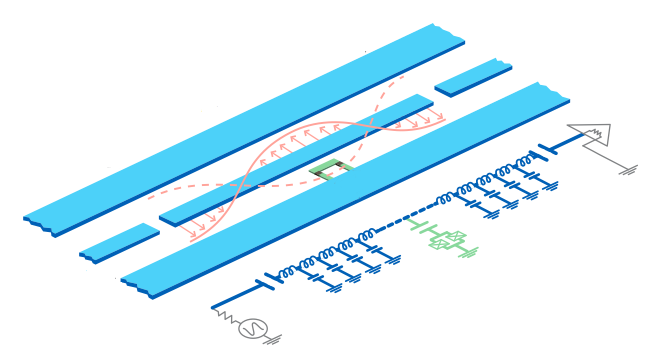
\includegraphics[width=3in]{SchustercQEDSchematic.png} 
   \caption{Schematic representation of cQED. The center pin is shown with an oscillating electromagnetic wave confined in the cavity. The capacitor gaps isolating the resonator act as mirrors containing the radiation. The cavity is coupled to a nearby qubit, here placed in the dielectric gap near the center of the resonator. A circuit schematic is also shown. Figure modified from \cite{Schuster}.}
   \label{fig:cQEDSchematic}
\end{figure}

A one-dimensional transmission line acts as the cavity\footnote{The terms cavity, resonator, transmission line, and waveguide are used interchangeably} within which photons propagate. The resonator is a conducting line separated from ground by a dielectric, as in a coaxial or fiber optic cable.The cavity resonant frequency is set by the length of the resonator between the two end capacitors.Typically, this is in the microwave regime\footnote{This is done to minimize thermal fluctuations affecting the circuit, as explained in Section \ref{sec:TransmissionLines}}. These capacitors act as mirrors, reflecting photons back and forth within the resonator. Vacuum conditions in the superconducting regime allow for remarkably low losses to be achieved.

Qubits are coupled to these transmission lines. To create quantum two-level systems, the typical electrical engineers toolbox is supplemented with the Josephson junction, the only known dissipationless non-linear circuit\cite{Devoret2004}. As shall be discussed in Sections \ref{sec:} and \ref{sec:}, a non-linear element is required to isolate two energy levels to serve as a computational qubit. Many different designs have been explored, in which different degrees of freedom operate as the computational basis states\footnote{For a good overview, see papers by ETC}. This is utilized for charge qubits such as the Cooper pair box\cite{Nakamura1999} relies upon the charge difference between capacitors created by quantum tunneling by superconducting Cooper pairs. The conjugate variable to charge, flux, may also been used. By storing flux quanta in a superconducting loop, the persistent current (or number of flux quanta) becomes the basis states for a viable qubit. Quantum phase is also a possible variable for computation. Each qubit design has its own strengths and weaknesses, such as being sensitive to different types of noise. %Each type of qubit has its own strengths and weaknesses, as summarized in Table \ref{tab:QubitTypes}. 

As in cavity QED, the composite qubit-resonator system reveals many interesting phenomena. Our chief method of realizing quantum information is via classical transmission measurements. By controlling the input and output of photons which interact with the superconducting qubits, we engineer ways to gain insight into the qubit states through familiar macroscopic parameters such as voltage and current. Typically, it is also possible to tune the qubit frequency into and out of resonance with the fixed cavity frequencies. Experiments, such as those in this thesis, rely on these two degrees of freedom. 

While this thesis does not explore any of the actual computational possibilities of the cQED architecture, multiple qubit-resonator buses may easily be coupled together to allow for the exchange and control of quantum information. CITE ARTICLE






%
%o	What is cQED: circuits based on cavity QED, ie. Realizing QED using superconducting circuits. 
%o	\cite{Blais} as starting the field
%o	“Electromagnetic signals are always composed of photons, although in the circuit domain those signals are carried as voltages and currents on wires, and the discreteness of the photon’s energy is usually not evident. However, by coupling a superconducting quantum bit to signals on a microwave transmission line, it is possible to construct an integrated circuit in which the presence or absence of even a single photon can have a dramatic effect.” \cite{Schuster Houck Resolving}
%o	Houck bullets
%•	Coupling qubits with photons
%•	Cavities enhance coupling, prevent information leakage
%•	Arbitrary pairwise coupling in one cavity
%•	Multiplexed readout and control
%o	Mirrored cavity suppresses decoherence
%o	Compress 2 dimensions of cavity to much less than a wavelength. This increases both the energy density and the dipole coupling. 
%o	\cite many papers, mention those that couple qubits together for actual computation (which I don’t cover)
%o	Low temperature → less thermal noise. If you think about the Boltzmann distribution, a really low temperature is required such that is prohibitively difficult to occupy the mode we are concerned with. At 20mK, the GHz regime corresponds to about 500mK, which is significantly greater



%Information is inherently a physical quantity, and the physics of information is the physics of all matter [Landauer1991]

\section{Outline}
Having given a brief introduction to quantum computing and cQED, this thesis continues in a much more focused manner. Chapter \ref{chap:Multimodal} presents the theoretical concepts investigated in this thesis: highly multimodal photon-qubit strong coupling in superconducting cQED circuits. To our knowledge, no work has been published in this field. However, this thesis is in part motivated by the theoretical work of Hakan T\"{u}reci and the unpublished Masters thesis of one of his students, Rafael Luger\cite{Luger}. This work, Spontaneous decay in the multi-mode regime of cavity quantum electrodynamics, describes a possible new regime in which a qubit may simultaneously couple to multiple modes of a cavity. This thesis presents initial experimental work into this regime. 

In order to understand these concepts, Chapter \ref{chap:Theoretical} presents an overview of topics standard to the literature. I feel it is most useful to understand the physics without getting too bogged down in the details of this particular thesis. As such, Chapter \ref{chap:Theoretical} is at a high level and should be applicable to any cQED system. I begin with the Jaynes-Cummings model as a prototypical cavity QED system, and explain the potential for this model to fit into the DiVincenzo criteria for quantum computing. From this, more advanced concepts are explored, such as nonlinear vacuum Rabi phenomena, cQED regimes, and more. 

Chapter \ref{chap:Implementing} discusses the actual implementations of building superconducting circuits. An effort is made to justify the higher level theory of Chapters \ref{chap:Theoretical} and \ref{chap:Multimodal} as we build the physics of these circuits from the ground up. This chapter is also specific to this thesis, and focuses almost exclusively on the particular cQED designs used. It discusses the transmission lines, transmon qubits, and the physics of coupling the two. 

Finally, Chapter \ref{chap:Experimental} reveals the methods and results of this thesis. ETC



%%%%%%%%%%%%%%%%%%%%%%%%%%%%%%%%%%%%%%%%%%%%%%%%%%
\chapter{Theoretical basis of cQED}\label{chap:Theoretical}
This chapter presents the standard theory behind circuit quantum electrodynamics. My intention is for this introduction to be applicable to the field of cQED as a whole, regardless of the nuances of any particular implementation. As such, I will discuss certain concepts broadly; for example, while the all the circuits built for this thesis contained transmon qubits, this chapter will discuss how any viable qubit fits into the general cQED architecture. A specific discussion of the implementations used in this thesis can be found in Chapter \ref{chap:Implementing}. Familiarity with the concepts of this chapter is required to understand the novel theoretical and experimental work undertaken for this thesis, as found in Chapter \ref{chap:Multimodal}. Those readers comfortable with the cQED literature are invited to skip ahead. 

I begin with the abstract requirements for quantum computation, as laid out in the DiVincenzo criteria. This serves to explain how and why cQED is a viable quantum computing architecture. The Jaynes-Cummings model is then used as a starting point to conceptualize cQED. I will then delve into some more complicated, but standard, topics such as Vacuum Rabi phenomena and coupling regimes.

\section{Architectural objectives}\label{sec:DiVincenzo}
Quantum computing is motivated by a clear purpose: the manipulation and control of quantum information. For any physical system to be a viable quantum computer it must meet a stringent set of requirements, as first set out by David DiVincenzo \cite{DiVincenzo}:

\begin{enumerate}
\item A well-defined unit of quantum information, i.e. good qubits. Any two quantum energy levels can be used as a computational quantum states, and as such many implementations have been pursued. Importantly, qubits need not be an actual atom; there are macroscopic systems that can act as a quantum two-level system. 
\item Reliable state preparation. The ability to initialize qubits into a computational null state is a necessary starting point for performing any kind of meaningful computation.
\item Low decoherence. Maintaining quantum states of information is notoriously difficult, yet imperative.  A major challenge is to engineer sufficiently long qubit relaxation ($T_1$) and dephasing ($T_2$) times as compared to the time scale of computation. 
\item Accurate quantum gate operations. Qubits must be able to interact with another in a controlled manner. 
\item Quantum non-demolition  measurements, i.e. the ability to read out the state of the system without destroying any information. 
\end{enumerate}

Circuit quantum electrodynamics is just one implementation that seeks to satisfy the above criteria. The genius of cQED lies in the use of quantized electromagnetic radiation to solve (4) and (5). We place qubits satisfying (1) and (2) into a cavity. We then add photons to the cavity in a controlled manner\footnote{In addition, the high speed of photons eases the constraint on engineering (3).}. These photons may interact with the qubit states, either by modifying the qubit state (4) or by performing a non-demolition measurement of the system (5). Coupling cavities together allows for the interaction of qubits via photons. Cavities are the quantum bus of the cQED architecture. Such a system is described by the Jaynes-Cummings model, a common theoretical model in quantum optics. 



%%%%%%%%%%%%%%%%%%%%%%%%%%%%%%%%%%%%%%%%%%%%%%%%%%%%%%%%%%%%%%%%%%%%%%%%%
\section{Jaynes-Cummings model}\label{sec:JC}
The Jaynes-Cummings model describes a two-level quantum system coupled to the quantized mode of an optical cavity. This cavity may or may not contain photons. The simplest model in CQED, it was originally proposed to study light-matter interaction, specifically the phenomenon of spontaneous emission. As opposed to a semi-classical theory, the Jaynes-Cummings model allows for an understanding of how the discrete nature of electromagnetic radiation affects the system. As such, it is the ideal starting point from which to examine cQED. Figure \ref{fig:ToycQED} presents a simplified visual diagram of the system.

\begin{figure}[h] 
   \centering
   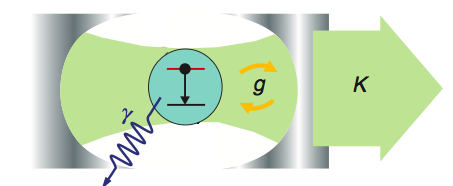
\includegraphics[width=3in]{Semba-Toy-cQED.png} 
   \caption{Jaynes-Cummings model. Green represents the EM field, blue represents the two-level quantum system and yellow the coupling between the two. The three rates $g$, $\kappa$ and $\gamma$ are schematically illustrated. In a cQED implementation, the cavity is replaced by a transmission line and the ``mirrors" shown are capacitors in the line. From \cite{Semba}.}
   \label{fig:ToycQED}
\end{figure}

Conceptually there are three main factors that describe the overall behavior of the system. First, the coupling between qubit and cavity modes is given by a rate constant $g$. This variable is dependent on numerous factors. Certain physical design considerations, such as the placement of the qubit in relation to the transmission line, are fixed for a particular circuit. As shall be mathematically described in Chapter \ref{sec:StrongCoupling}, the transition frequency of the qubit may be tuned in and out of resonance with the modes of the cavity. The tuning affects the coupling rate $g$. 

As no system is perfect, there are two main sources of decoherence. While we think of the walls of the cavity as ``mirrors," photons will leak out at a rate $\kappa$. Similarly, driving the addition of photons into the cavity is limited by the same rate. This term is determined by the engineering of the capacitors that enclose the resonator, as will be detailed in Chapter \ref{chap:Implementing}. 

The $\gamma$ term gives an all-encompassing rate for decoherence that may be experienced by the qubit. This relates directly to $T_1$ and $T_2$ times for the system; we can approximate $O(1/\gamma)= O(T_1,T_2)$. INCLUDE SPONTANEOUS EMISSION. As a qubit may be in a quantum superposition of states, it precesses, acting as a sort of clock measuring the frequency difference between the two states. If the qubit is subject to noise (internal or external) the clock can lose time or dephase, a subtle form of decoherence.\cite{Schuster} This form of decoherence occurs at the dephasing rate $T_2$.

Turning to the physics of the model, the Jaynes-Cummings Hamiltonian is given by

\begin{equation}\label{eq:JC}
H=\hbar \omega_r(a^\dag a + \frac{1}{2}) + \frac{1}{2}\hbar \omega_a \sigma_z + \hbar g(a^\dag \sigma_- + a\sigma_+)
\end{equation}

for a single cavity mode of frequency $\omega_r$.\footnote{The Jaynes-Cummings model is limited to describing a single photon mode. As in the cQED literature, this chapter defines the mode $\omega_r$ as the lowest harmonic of the cavity. } This follows the simplfied form

\begin{equation}
H_{\mathrm{JC}} = H_{\mathrm{field}}+H_{\mathrm{atom}}+H_{\mathrm{int}}
\end{equation}

While it is imperative that the system be considered as a whole, I shall briefly describe the meaning of the three terms. Chapter \ref{chap:Implementing} will prove that the constituent parts of the cQED architecture are accurately described by these terms. 

%%%%%%%%%%%%%%%%%%%%%%%%%%%%%%%%%%%%%%%%%%%%%%%%%%
\subsection{Cavity modes}
Transmission lines in cQED act as quantized harmonic oscillators. As such, the possible frequencies of quantized EM radiation are dependent on the fundamental frequency of the cavity. These are closely related to integer multiples of twice the cavity length. This gives a linear spectrum of available frequencies. A quantized harmonic oscillator is described by 

\begin{equation}\label{eq:CavityHamiltonian}
H_{\mathrm{field}}=\hbar \sum_n\omega_n(a_n^\dag a_n+\frac{1}{2})
\end{equation}

for all possible frequencies. The raising and lowering operators work in the standard way

\begin{equation}
a^\dag\ket{n}=\sqrt{n+1}\ket{n+1} \hspace{1.3cm} a\ket{n}=\sqrt{n}\ket{n-1} 
\end{equation}

such that $a^\dag a\ket{n}=n\ket{n}$ reveals the number of photons in the cavity. However, we are often interested in the behavior of the circuit for one particular frequency. The case for the single resonant  frequency $\omega_r$ simplifies to 

\begin{equation}
H_{\mathrm{field}}=\hbar \omega_r(a^\dag a+\frac{1}{2})
\end{equation}

As such, we define the state of the cavity by $\ket{n}$, for $n \in \mathbb{Z}$.

%%%%%%%%%%%%%%%%%%%%%%%%%%%%%%%%%%%%%%%%%%%%%%%%%%
\subsection{Qubit excitations}
As a two-level quantum system, the qubit has a ground state $\ket{g}$ and excited state $\ket{e}$. The transition energy $\hbar \omega_a$ between the two states is defined in terms of a frequency $\omega_a$. For the term $H_{\mathrm{atom}}$ to describe this physically we co-opt the two-dimensional Pauli inversion operator $\sigma_z$

\begin{equation}
\sigma_z\ket{g}=-\ket{g} \hspace{1.3cm} \sigma_z\ket{e}=\ket{e}
\end{equation}

so that $H_{\mathrm{atom}}$ acting on the system gives eigenenergies $E_g=-\hbar\omega_a/2$ and $E_e=\hbar\omega_a/2$. The difference in energy between the two states is satisfied. 

%%%%%%%%%%%%%%%%%%%%%%%%%%%%%%%%%%%%%%%%%%%%%%%%%%
\subsection{Emission and absorption}\label{sec:Emission}
EXPLAIN DIPOLE COUPLING
The final term $H_{\mathrm{int}}$ gives the energy of the dipole coupling between the qubit and cavity field.\footnote{This term is implicitly defined as being in the Rotating Wave approximation, which will be justified in Chapter \ref{chap:Implementing}.} The two possible interactions are the simultaenous annihilation of a photon and excitation of the qubit, $a\sigma_+$, as well as the inverse, $a^\dag \sigma_-$. We use the Pauli raising and lowering operators to describe the excitations of the qubit

\begin{eqnarray}
\sigma_+\ket{g} = \ket{e} \hspace{1.3cm} \sigma_-\ket{g} = \ket{0} \\
\sigma_+\ket{e} = 0\hspace{1.3cm} \sigma_-\ket{e} = \ket{g} \nonumber
\end{eqnarray}

Note that the creation operator acting on the excited state, as well as the annihilation operator acting on theground state, produces $\ket{0}$. As expected, each subspace has only two distinct energy levels and therefore the coupling term $H_{\mathrm{int}}$ only connects the states $\ket{n,g}$ and $\ket{n-1,e}$.

By coupling the qubit and cavity modes there exist two tunable frequencies, $\omega_r$ of the cavity and $\omega_a$ of the qubit. Whether by engineering the length of the cavity to specific dimensions or tuning the qubit frequency $in$ $situ$, we can tune the frequencies into resonance with one another. This is defined by

\begin{equation}
\Delta = |\omega_r - \omega_a|
\end{equation}

As stated in Chapter \ref{sec:JC}, the tuning parameter $\Delta$ affects the rate of coupling $g$. It also defines the regimes in which cQED can be operated, each of which gives rise to unique phenomena and can be used for different purposes. 

%%%%%%%%%%%%%%%%%%%%%%%%%%%%%%%%%%%%%%%%%%%%%%%%%%
\section{Quantum states}
With the Jaynes-Cummings model, we now understand how to parametrize the state of our system. A cQED circuit for a single cavity mode is described in two dimensions: (1) the qubit excitation state and (2) the number of photons in the cavity. We therefore describe the state of the entire system by a composite vector of the two subspaces. For example, the ground state of the entire system is given by $\ket{0,g}$, for which the qubit is in the ground state $g$ and there are no photons of the given frequency inside the cavity. 

This allows us to obtain a matrix representation of the Hamiltonian (\ref{eq:JC}) 

\begin{equation}\label{eq:Matrix}
H =  \hbar\left(\begin{array}{cccccccc}
%\ket{0,g}  & \ket{1,g} & \ket{0,e} & \ket{2,g} & \ket{1,e} & ... &\ket{n,g} & \ket{n-1,e}\\
0 \\
& \omega_r 	& g \\
& g    		& \omega_a \\
&&&2\omega_r	 & \sqrt{2}g \\
&&&\sqrt{2}g 		& \omega_r + \omega_a\\
&&&&&\ddots\\
&&&&&&n\omega_r & \sqrt{n}g\\
&&&&&&\sqrt{n}g    & (n-1)\omega_r+\omega_a
\end{array} \right)
\end{equation}

by expressing it in the basis of the excitation subsystems

\begin{equation}
\left(\begin{array}{cccccc} \ket{0,g} & \ket{1,g} & \ket{0,e} & ... & \ket{n, g} & \ket{n-1,e}
\end{array}\right)
\end{equation}

The coupling term causes the matrix to be block diagonal by only connecting the states $\ket{n,g}$ and $\ket{n-1,e}$. With the exception of the ground state, we can examine any 2-by-2 submatrix to analytically solve for the $n^{th}$ excitation manifold

\begin{equation}
\left(\begin{array}{cc}
\matrixel{n,g}{H}{n,g} & \matrixel{n-1,e}{H}{n,g} \\
\matrixel{n,g}{H}{n-1,e} & \matrixel{n-1,e}{H}{n-1,e}
\end{array}\right) = \hbar \left(\begin{array}{cc}
n\omega_r-\frac{1}{2}\Delta 	& g\sqrt{n} \\
 g\sqrt{n}					& n\omega_r+\frac{1}{2}\Delta
\end{array}\right)
\end{equation}

which yields the ``dressed" eigenstates\footnote{The variable $\theta_n$ satisfies $\tan{2\theta_n}=\frac{2g\sqrt{n}}{\Delta}$} 

\begin{eqnarray}
\ket{n_+} &=& \sin(\theta_n)\ket{n,g}+\cos(\theta_n)\ket{n-1,e} \\
\ket{n_-} &=& \cos(\theta_n)\ket{n,g}-\sin(\theta_n)\ket{n-1,e}
\end{eqnarray}

with corresponding energies

\begin{eqnarray}
E_0/\hbar &=& -\frac{\Delta}{2} \\
E_n/\hbar &=& n\omega_r \pm \frac{1}{2}\sqrt{4ng^2+\Delta^2} \nonumber
\end{eqnarray}

%As quantum computing is exceptionally sensitive to decoherence, any loss of information is a threat to maintaining quantum information. The strong coupling regime describes the ideal dynamics by which to solve such a problem. It is relatively easy for cQED architecture to realize this regime, a major reason this field is at the forefront of research into quantum computing. 

%%%%%%%%%%%%%%%%%%%%%%%%%%%%%%%%%%%%%%%%%%%%%%%%%%%%%%%%%%%%%%%%%%%%%%%
\section{Nonlinear Vacuum Rabi phenomena}\label{sec:Rabi}
Resonance, defined as tuning the cavity and resonator frequencies to be equal $\Delta=0$, leads to some truly remarkable phenomena in cQED systems. First, note that in the $\emph{uncoupled}$ resonant case $\omega_r=\omega_a$ the separate cavity and qubit systems both have a linear energy level spectrum $E_n=n\omega_{r,a}$, as expected for a simple harmonic oscilator. A transmission measurement of a bare cavity will reveal the linearity of the resonant frequencies, as modelled in Fig. (\ref{fig:Transmission1}).

\begin{figure}[h] 
   \centering
   
\includegraphics[width=2.5in]{placeholder.jpg} 
   \caption{Left: Model of the transmission spectrum of a bare cavity. Higher order harmonics are integer multiples of resonant frequency $\omega_r$. The linewidth ETC. Right: Model of the transmission spectrum of a coupled cavity-qubit system at resonance. The ETC}
   \label{fig:Transmission1}
\end{figure}

However, resonance creates degeneracy in a coupled system. This can be observed by solving the Hamiltonian (\ref{eq:JC}) in the resonant limit. More specifically, so long $\Delta=|\omega_a-\omega_r|<<g$ we make the approximation $\omega_a=\omega_r$.\footnote{It's impossible for any lab setup to achieve perfection!} For a general subsystem of $n$ photons

\begin{equation}
H_n = \hbar \left( \begin{array}{cc}
n\omega{r} & \sqrt{n}g \\
\sqrt{n}g & n\omega_r
\end{array}\right)
\end{equation}

we solve to find nonlinear energy eigenvalues

\begin{equation}\label{eq:NonlinearEnergies}
E_n = \hbar(n\omega_r\pm \sqrt{n}g)
\end{equation}

and simplified dressed eigenstates

\begin{equation}
\ket{n_{+,-}} = \frac{\ket{n,g}\pm\ket{n-1,e}}{\sqrt{2}}
\end{equation}

Thus, coupling the atomic and cavity subsystems lifts the degeneracy by $2\sqrt{n}g$ at each energy level. a phenomena referred to as \emph{Vacuum Rabi splitting}. This creates an effective two-level system between the ground state $\ket{0,g}$ and antisymmetric eigenstate of the first excitation manifold $\ket{n_-}$, in which the transition energy between the two states is less than $\omega_r$. Fig. (\ref{fig:EnergyLevels}) shows both the degenerate and hybridized energy levels. 

\begin{figure}[h] 
   \centering
   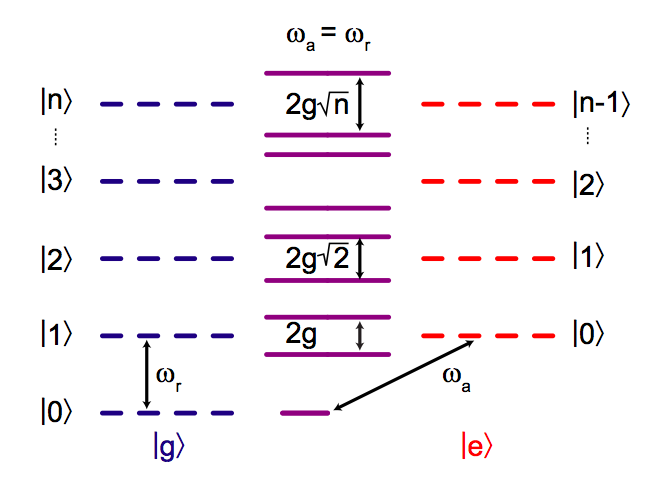
\includegraphics[width=4in]{SchusterResonantEnergyLevels.png} 
   \caption{Energy level diagrams of the Jaynes-Cummings Hamiltonian. From \cite{Schuster}.}
   \label{fig:EnergyLevels}
\end{figure}

A transmission measurement of the resonant, coupled system will show two transmission peaks around the resonant frequency $\omega_r$, one for each new eigenstate. Appropriately, this conveys the difference in eigenenergies, as the frequency splitting is $E_n/\hbar=2\sqrt{n}g$. PEAK WIDTHS? AFFECTS QUBIT STATE, HOW IS THIS DIFFERENT FROM DISPERSIVE MEASUREMENT?

In cQED the atom cannot be physically removed from the cavity to switch off the vacuum Rabi splitting —instead the atom is tuned far away from the cavity in frequency space. Vacuum Rabi splitting is thus typically observed in the form of an avoided crossing, occurring as the qubit frequency is tuned through resonance with the cavity\cite{Bishop}. Amazingly, at resonance the two frequencies $\omega_r$ and $\omega_a$ are never equal, despite the definition of resonance $\omega_r=\omega_a$. Coupling the system actually affects the modes of each individual subsystem. They will always differ by a frequency of at least $2\sqrt{n}g$. As $\Delta$ moves away from resonance, the states revert back to their unmixed form. An example of an avoided crossing is shown in Figure (\ref{fig:AvoidedCrossing}).

\begin{figure}[h] 
   \centering
   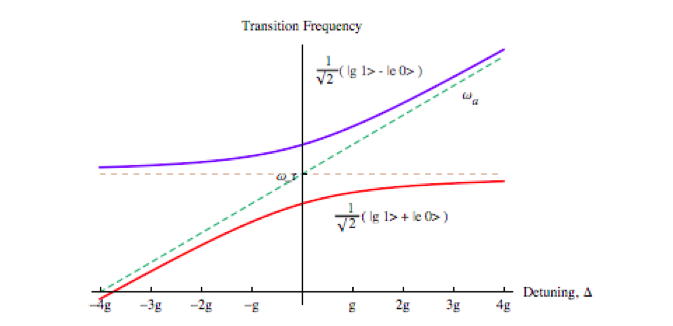
\includegraphics[width=5in]{ElizaAvoidedCrossing.png} 
   \caption{FIX TO BE GENERAL}
   \label{fig:AvoidedCrossing}
\end{figure}

As the two eigenstates $\ket{n_+}$ and $\ket{n_-}$ differ in energy, a system will precess between the two states at the rate $2\sqrt{n}g$

\begin{equation}
\ket{\psi(t)}=\ket{n_-}+\ket{n_+}e^{i2\sqrt{n}gt}
\end{equation}

Equivalently, this can be seen as an oscillation between our original basis states. Thus, any system placed in the pure state $\ket{n,g}$ will oscillate back and forth to $\ket{n-1,e}$. This oscillation between states is known as \emph{Vacuum Rabi oscillations}. 

%%%%%%%%%%%%%%%%%%%%%%%%%%%%%%%%%%%%%%%%%%%%%%%%%%%%%%%%%%%%%%%%%%%%
\section{Anharmonicity: Climbing the Jaynes-Cummings ladder}\label{sec:Anharmonicity}
Vacuum Rabi behavior is not proof of Jaynes-Cummings physics, as pointed out by Zhu \emph{et al.}\cite{Zhu} and Tian \emph{et al.}\cite{Tian}. Coupled classical harmonic oscillators can display the same hybridized mode splitting at resonant frequencies. However, resonant coupling also introduces a larger scale anharmonicity that is a uniquely quantum effect. Returning to  Eq. (\ref{eq:NonlinearEnergies}), energy levels at resonance are predicted to scale by the power law $n^{1/2}$ with the number of excitations $n$ of the system. This quantum effect is in stark contrast to the normal mode splitting of two classical couplied linear oscillators, which is independent of oscillator amplitude\cite{Fink}. This can be seen as a photon-photon interaction; introducing another photon to the system is dependent on the number of photons already in the cavity. This anharmonic behavior has been observed using Rydberg atoms in microwave cavities \cite{}, two-tone pump probe measurements \cite{Fink}, and for time-domain measurements of phase qubits \cite{Hofheinz, Wang}.
MORE? ANY DERIVATIONS?

%%%%%%%%%%%%%%%%%%%%%%%%%%%%%%%%%%%%%%%%%%%%%%%%%%%%%%%%%%%%%%%%
\section{cQED Regimes} %Or dispersive limit?
Circuit quantum electrodynamics can be characterized by a number of regimes. While this thesis is focused on effects seen in the strongly resonant limit, other regimes are of interest and necessary for experimental work. Typically, these regimes are determined by two parameters, strong vs. weak and resonant vs. dispersive (i.e. tuning $\Delta$). Fig. \ref{fig:Regimes} gives an overview of the parameter space. 

\begin{figure}[h] 
   \centering
   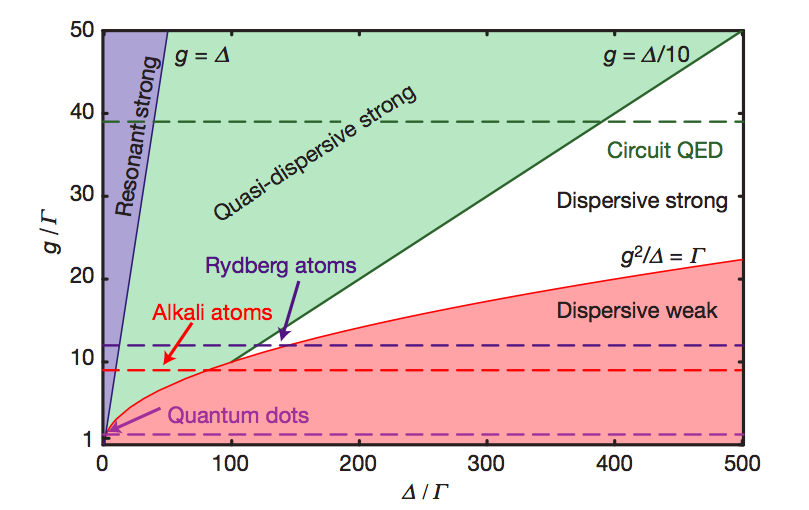
\includegraphics[width=5in]{HouckParameterSpace.png} 
   \caption{CAPTION. Figure from \cite{SchusterResolving}.}
   \label{fig:Regimes}
\end{figure}

%%%%%%%%%%%%%%%%%%%%%%%%%%%%%%%%%%
\subsection{Strong coupling}\label{sec:StrongCoupling}
Strong coupling is defined as 

\begin{equation}
g>>[\gamma, \kappa]
\end{equation}

for which a single qubit can absorb and re-emit a single photon many times before decay. Recall that $g$ is the rate of coupling between the qubit and cavity. I

DOES THIS EXPLAIN INCREASING RATE OF COUPLING FOR EVERY PHOTON OSCILLATION, OR IS IT REALLY DECREASING DECOHERENCE??


%%%%%%%%%%%%%%%%%%%%%%%%%%%%%%%%%%
\subsection{Dispersive Limit}
Resonance has already been defined as $\Delta << g$; in the ideal case, $\Delta=0$. The dispersive limit is achieved by significant atom cavity detuning, $\Delta=|\omega_a-\omega_r| >> g$. Perturbation theory allows us to expand the Hamiltonian (\ref{eq:JC}) in powers of $g/\Delta$ to second order

\begin{eqnarray}
H&=&\hbar \omega_r\left(a^\dag a + \frac{1}{2}\right) + \frac{1}{2}\hbar \omega_a \sigma_z + \hbar g(a^\dag \sigma_- + a\sigma_+) \\
&\approx& \hbar\omega_r \left( a^\dag a +\frac{1}{2}\right)+\frac{1}{2}\hbar\sigma_z\left(\omega_a+\frac{2g^2}{\Delta}a^\dag a +\frac{g^2}{\Delta}\right) \label{eq:Dispersive}
\end{eqnarray}

which can be rewritten as 

\begin{equation}
H\approx \hbar\left( \omega_r+\frac{g^2}{\Delta}\sigma_z\right) \left(a^\dag a+\frac{1}{2}\right)+\frac{1}{2}\hbar\omega_a\sigma_z\label{eq:DispersiveQND}
\end{equation}

Eqs. (\ref{eq:Dispersive}) and (\ref{eq:DispersiveQND}) are the same, yet they give different insights into the system. Eq. (\ref{eq:Dispersive}) maintains the nature of the cavity, instead highlighting a shift in the qubit's frequency. The qubit is modified by both a photon number-dependent ``Stark" shift ($2ng^2/\Delta$) and a vacuum noise induced ``Lamb" shift ($g^2/\Delta$). Physically when the atom state is changed it must electrically compress (or expand) the photons' wavelength, increasing (or decreasing) the frequency of each photon in the cavity, which will require extra energy ($\hbar g^2/\Delta$).

The equation is grouped to show the effect of the dispersive limit on the qubit's behavior. The qubit frequency undergoes a ``light" shift consisting of a photon number-dependent ``Stark" shift ($2ng^2/\Delta$) and a resonator vacuum induced ``Lamb" shift ($g^2/\Delta$)\cite{Schuster}. The latter shows the effect of coupling the subsystems even in the absence of excitations. The Stark shift term shows that, even in the dispersive limit, photon-qubit coupling will modify the state of the two-level system. 

Eq. (\ref{eq:DispersiveQND}) shifts focus onto the behavior of the resonator. The cavity experiences a frequency shift $\chi=g^2/\Delta$ dependent on the state of the qubit, $\sigma_z$. Thus, both the cavity and qubit experience frequency shifts subject to detuning by the power law $\Delta^{-1}$; this shows the gradual effects of tuning the qubit in and out of resonance\footnote{Note that this term only holds for the dispersive limit. In the resonant regime, $\Delta^{-1}$ does not apply, or else we'd have infinite frequency shifts!}. This is diagrammed in Fig. (\ref{fig:DispersiveEnergyLevels})

\begin{figure}[h] 
   \centering
   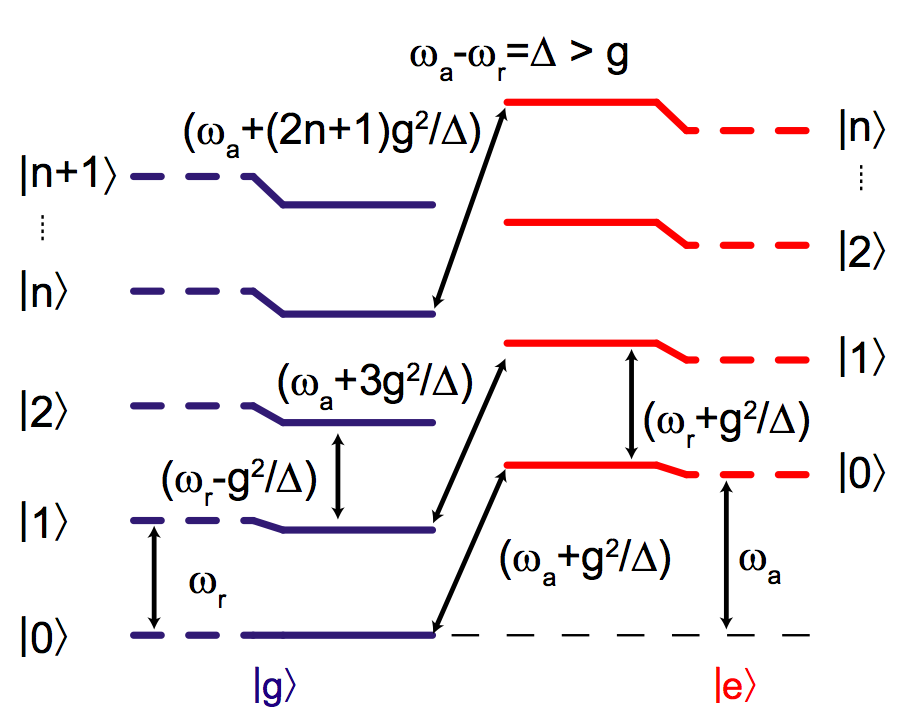
\includegraphics[width=2in]{SchusterDispersiveEnergyLevels.png} 
   \caption{ADD CAPTION. From \cite{Schuster}.}
   \label{fig:DispersiveEnergyLevels}
\end{figure}

The simultaneous dispersive shifts of both the qubit and resonator allows for Quantum non-demolition (QND) measurements in the strong limit, a necessary requirement from Chapter \ref{sec:DiVincezo}. Unlike in the resonant case, the frequency shifts for each subsystem are individual in nature, even if they are connected. A transmission measurement of resonant system will show the state of the qubit based upon the shift from $\omega_r$, however it acts as a direct measurement of the qubit and thus affects its state.

In the dispersive regime, the problem of determining the frequency of the qubit is rephrased to determining the bare resonator frequency (since this is different from any possible qubit frequency). For  Probing the system at this specific frequency, we can infer the state of the qubit! In the case that $\chi<\kappa$, multiple photons can be used to increase the gain of the measurement. As such, the dispersive regime is used for measurements of cQED systems. 

Conversely, measuring the state of the qubit will can provide information about the cavitys frequency. When the Stark shift $\chi$ exceeds the qubit decay $\gamma$, the qubit frequency is shifted by more than the linewidth of the transmission peak. As such, each individual photon mode is reflected in a distinct qubit frequency. While this is never computationally useful, it reflects a duality in the effects each of the two subsystems experiences. Fig. (\ref{fig:DispersiveStrong}) shows the behavior of all frequency shifts in the strong dispersive regime. 

\begin{figure}[h] 
   \centering
   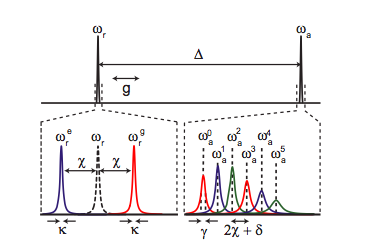
\includegraphics[width=4in]{SchusterDispersiveFrequencyShifts.png} 
   \caption{ADD CAPTION. From \cite{Schuster}.}
   \label{fig:DispersiveFrequencyShifts}
\end{figure}

%%%%%%%%%%%%%%%%%%%%%%%%%%%%%%%%%%%%%%%%%%%%%%%%%%%%%%%%%%%%%%%%%%%%%%%%%%%%
%%%%%%%%%%%%%%%%%%%%%%%%%%%%%%%%%%%%%%%%%%%%%%%%%%%%%%%%%%%%%%%%%%%%%%%%%%%%
%%%%%%%%%%%%%%%%%%%%%%%%%%%%%%%%%%%%%%%%%%%%%%%%%%%%%%%%%%%%%%%%%%%%%%%%%%%%
\chapter{Highly multimodal photon-qubit strong coupling}\label{chap:Multimodal}

We expand the first excitation subsystem of the Jaynes-Cummings Hamiltonian (\ref{eq:Matrix}) to demonstrate new multimodal behavior

\begin{equation}\label{eq:Matrix}
H_1 =  \hbar\left(\begin{array}{cc}
\omega_r 	& g \\
g    		& \omega_a 
\end{array} \right)
\end{equation}

The basis states are

\begin{equation}
\left(\begin{array}{cccccc} \ket{0,g} & \ket{1,g} & \ket{0,e} & ... & \ket{n, g} & \ket{n-1,e}
\end{array}\right)
\end{equation}

The Jaynes-Cummings Hamiltonian has been implicitly been working with $n$ photons of frequency $\omega_r$. We now define $\omega_r$ to be the fundamental mode of the cavity, $m=1$. The variable $m$ will denote the harmonics of the modes for the quantum state. This differentiates between the second mode $m=2$ of a resonator of length $d$ and the fundamental mode $m=1$ for a resonator of length $d/2$, despite the two modes having the same frequency. This is necessary because the two resonators have drastically different mode spacings $\delta\omega_r$. 

Having introduced the mode quantum number $m$, we write the quantum state of the system for the number of photons $n$ of mode $m$ for the fundamental resonator frequency $\omega_r$, with a qubit of transition frequency $\omega_a$ state $g$ or $e$

\begin{equation}
\ket{n,m,g} \hspace{0.7cm} \mathrm{or} \hspace{0.7cm} \ket{n,m,e}
\end{equation}

There is now a more complicated system of photon-qubit interaction. AT RESONANCE? In resonance, $\Delta=0$, there is still the regular method of qubit excitation/photon annihilation, and its inverse

\begin{equation}
\matrixel{n-1,e}{H}{n,g} =\matrixel{n,g}{H}{n-1,e} =\sqrt{n}g
\end{equation}

provided that the qubit frequency $\omega_a$ and the frequency of the photon causing the excitation are equivalent, i.e. the photon frequency is implicitly the fundamental mode $\omega_r$


%%%%%%%%%%%%%%%%%%%%%%%%%%%%%%%%%%%%%%%%%%%%%%%%%%%%%%%%%%%%%%%%%%%%%%%%%%%%
%%%%%%%%%%%%%%%%%%%%%%%%%%%%%%%%%%%%%%%%%%%%%%%%%%%%%%%%%%%%%%%%%%%%%%%%%%%%
%%%%%%%%%%%%%%%%%%%%%%%%%%%%%%%%%%%%%%%%%%%%%%%%%%%%%%%%%%%%%%%%%%%%%%%%%%%%
\chapter{Implementing cQED with superconducting circuits}\label{chap:Implementing}
Having discussed circuit quantum electrodynamics at a high level in Chapters \ref{chap:Theoretical} and \ref{chap:Multimodal}, we now turn to the engineering of such a system out of circuits. In discussing the physical implementation taken in this thesis, particular attention is paid to justifying the use of the Jaynes-Cummings model as a starting point for the previous chapters. The actual methods used to fabricate each device is discussed in Chapter \ref{chap:Experimental}

The circuits designed for this thesis are, as compared to the field in general, relatively simple designs. They consist of a single extremely long transmission line resonator capacitively coupled to input and output lines. A single transmon qubit, an advanced form of a Cooper pair box charge qubit, is placed near the end of the resonator. These circuits are refrigerated and operated at approximately 20mK temperatures. As such, we first begin with some relevant theory on superconductivity. 

%%%%%%%%%%%%%%%%%%%%%%%%%%%%%%%%%%%%%%%%%%%%%%%%%%%%%%%%%%%%%%%%%%%%
\section{Superconductivity}

%%%%%%%%%%%%%%%%%%%%%%%%%%%%%%%%%%%%%%%%%%%%%%%%%%%%%%%%%%%%%%%%%%%%
\section{Transmission lines}\label{sec:TransmissionLines}
USE GOPPL PAPER

Transmission lines form the resonators of the cQED architecture. Superconductors are used to minimize dissipative losses. The circuits in this thesis were constructed using niobium wafers on sapphire substrate.

Certain design considerations must be taken in to account in building superconducting resonators. Current equipment will cool equipment  to approx. 20mK, i.e. $k_BT\approx2.76*10^{-28}$ joules. In considering potential sources of decoherence, it is important that the circuit (including the qubit) operate at a significantly higher energy scale than the thermal bath, or else random fluctuations are likely to destroy any coherent behavior. The higher end of the microwave spectrum, i.e. the GHz regime, corresponds to approx. 250mK temperatures, i.e. $k_BT\approx3.45*10^{-27}$. Using simple Boltzmann statistics, the potential for an unwanted transition due to thermal fluctuations is sufficiently negligible

\begin{equation}
e^{-\frac{3.45*10^{-27}}{2.76*10^{-28}}}=?????
\end{equation}

Thus we operate cQED in the microwave regime. Happily, our lab equipment allows for frequency sweeps from 4-11 GHz. This fixes the general length scales of the resonator. ETC CALCULATE



\begin{figure}[h] 
   \centering
   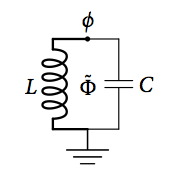
\includegraphics[height=3cm]{BishopLC.png} 
   \caption{ADD CAPTION. Figures \cite{Bishop}.}
   \label{fig:LCOscillator}
\end{figure}

To describe a quantized transmission line resonator, we begin with the textbook LC oscillator\footnote{Both \cite{Bishop} and \cite{Schuster}, being far better electrical engineers than I, also give a thorough treatment of the circuit from a classical starting point.}. This simple circuit, shown in Fig. (\ref{fig:LCOscillator}) consists of a inductor $L$ and capacitor $C$ connected in a loop. The circuit is used to store electrical energy oscillating at its resonant frequency. The inductor stores energy in its magnetic field, dependent on the current through the inductor. The voltage between the capacitor plates determines the energy stored in its electric field. Energy oscillates back and forth between the two units, creating an idealized dissipationless resonator. As we are operating at superconducting temperatures, we assume no resistance. The resonant frequency is determined by tuning the inductor and capacitor

\begin{equation}
\omega = \sqrt{\frac{1}{LC}}
\end{equation}

As a resonator, the LC circuit has quantum Hamiltonian identical in form to that of a simple harmonic oscillator. The two conjugate variables are the flux $\phi$ (from the inductor) and charge $q$ (from the capacitor)

\begin{equation}\label{eq:LCHamiltonian}
H=\frac{q^2}{2C}+\frac{\phi^2}{2L}
\end{equation}

Defining the impedance as

\begin{equation}
Z=\sqrt{\frac{L}{C}}
\end{equation}

we can introduce creation and annihilation operators obeying 

\begin{eqnarray}
\phi=\sqrt{\frac{\hbar Z}{2}}\left(a+a^\dag\right) \\
q=-i\sqrt{\frac{\hbar}{2Z}}\left(a-a^\dag\right)
\end{eqnarray}

with the commutation relation $[a,a^\dag]=1$. This formulates the Hamiltonian (\ref{eq:LCHamiltonian}) as a measure of the excitations of the circuit

\begin{equation}\label{eq:SHO}
H=\hbar \omega\left(a^\dag a + \frac{1}{2}\right)
\end{equation}

The relationship between the canonical ``position" and ``momentum" variables is described by 

\begin{eqnarray}
\frac{\partial H}{\partial q}=\frac{q}{C}=-L\frac{\partial I}{\partial t}=-\dot{\phi} \label{eq:Hpartial}\\
\frac{\partial H}{\partial \phi}=\frac{\phi}{L}=I=\dot{q}
\end{eqnarray}

A continuous chain of LC oscillators may be used to describe a transmission line beyond the lumped element approximation\cite{Pozar}. This is necessary for a circuits with dimensions on the same order as the electromagnetic wavelengths of interest. Following the derivation of \cite{Bishop}, we build a transmission line of length $d$, capacitance per unit length $c$ and inductance per unit length $l$. We use Eq. (\ref{eq:Hpartial}) to rewrite the Hamiltonian (\ref{eq:LCHamiltonian}) as a single-variable Lagrangian

\begin{equation}
L(\phi, \dot{\phi})=\frac{C\dot{\phi}^2}{2}-\frac{\phi^2}{2L}
\end{equation}

\begin{figure}[h] 
   \centering
   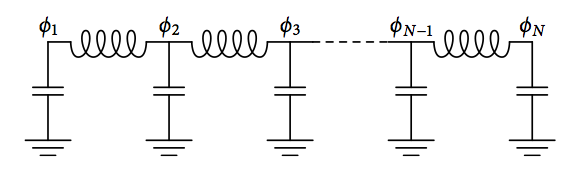
\includegraphics[width=3in]{BishopLCChain.png} 
   \caption{A transmission line resonator as an infinite chain of discrete LC oscillators. Figures \cite{Bishop}.}
   \label{fig:LCChain}
\end{figure}

A chain of $N$ oscillators spanned by the inductor components, as seen in Fig. (\ref{fig:LCChain}) is described by 

\begin{equation}\label{eq:LCLagrangian}
L(\phi_1, \dot{\phi}_1,...,\phi_N, \dot{\phi}_N)=
\sum_{i=1}^N \frac{\Delta C \dot{\phi_i}^2}{2} -
\sum_{i=1}^{N-1}\frac{(\phi_{i+1}-\phi_i)^2}{2\Delta L}
\end{equation}

for which the capitance and inductance are broken down per unit length by $\Delta C=cd/N$ and $ld/N$, respectively. Letting $N\rightarrow \infty$, Eq. (\ref{eq:LCLagrangian}) becomes an integral over the length of the circuit

\begin{equation}\label{eq:LCLagrangianIntegral}
L[\phi(x,t),\dot{\phi}(x,t)]=
\int_0^d\frac{c\dot{\phi}(x,t)^2}{2}-\frac{1}{2l}\left(\frac{\partial\phi(x,t)}{\partial x}\right)^2\mathrm{d}x
\end{equation}

The corresponding Euler-Lagrange equation

\begin{equation}
\frac{\partial^2\phi}{\partial t^2}=v^2\frac{\partial^2\phi}{\partial^2 x}
\end{equation}

describes the dynamics of the circuit in the flux basis, revealing a wave velocity of $v=1/\sqrt{lc}$. The general solution is

\begin{equation}\label{eq:ELSolution}
\phi(x,t)=\sum_{n=1}^\infty A_n\cos(k_nx+\alpha_n)\cos(k_nvt+\beta_n)
\end{equation}

Open circuit boundary conditions are described by 

\begin{equation}
\frac{\partial\phi}{\partial x}\bigg|_{x=0}=\frac{\partial\phi}{\partial x}\bigg|_{x=d}=0
\end{equation}

which solves for $\alpha_n=0$ and the wave number $k_n=n\pi/d$. Combining this with the wave velocity, we find that our circuit has resonant frequency modes $\omega_n=nv\pi/d$. Substituting Eq. (\ref{eq:ELSolution}) into the Lagrangian (\ref{:LCLagrangianIntegral})  yields 

\begin{equation}
L(\Phi_1, \dot{\Phi_1})=\sum_{n=1}^\infty\frac{C_n\dot{\Phi_n}^2}{2}-\frac{\Phi_n^2}{2L_n}
\end{equation}

$\Phi_n(t)=A_n\cos(k_nvt+\beta_n)$ is the final time-dependent solution, with effective capacitances $C_n=cd/2$ and inductances $L_n=2dl/n^2\pi^2$. Using the inverse of the original transform (\ref{eq:Hpartial}), we recover the quantum Hamiltonian for an extended transmission line resonator 

\begin{equation}
H=\hbar\sum_n \omega_n (a^\dag_n a_n + \frac{1}{2})
\end{equation}

This Hamiltonian reflects the infinite, linear spectrum of mode frequencies that can exist in the cavity. Each individual mode behaves as a harmonic oscillator; the modification from (\ref{eq:SHO}) is the creation of a ladder of resonant modes.

 So far, our discussion of the circuit has been centered on the quantum variables $\phi$ and $q$. These terms describe the discrete nature of the possible electromagnetic excitations that may exist in the cavity. Remarkably, the resonator is sensitive to the existence of even a single photon. 

%%%%%%%%%%%%%%%%%%%%%%%%%%%%%%%%%%%%%%%%%
\subsection{Coplanar waveguide cavities}
GOPPL PAPER
This thesis used coplanar waveguide (CPW) geometry in constructing superconducting transmission line circuits. While other options exist, the CPW design places ground in the same plane as the transmission line, separated by a dielectric gap. 

The transmission line, shown in Fig. (\ref{fig:CPW}) as having width $a$, 


%%%%%%%%%%%%%%%%%%%%%%%%%%%%%%%%%%%%%%%%%%%%%%%%%%%%%%%%%%%%%%%%%%%%
\section{Transmons}
As discussed in Section \ref{sec:DiVincenzo}, the qubit is designed to be a two-level system. I have already shown that quantized harmonic oscillators have a infinite, linear spectrum of energy levels. It is therefore impossible to isolate any two energy levels as computational basis states, such that driving a transition between these two levels will not also populate other, erroneous energy levels. 

A two-level quantum system is achieved by introducing anharmonicity. While an anharmonic circuit is not strictly two-level, as many energy levels exist, a good superconducting qubit is designed to have sufficient anharmonicity such that it is effectively two-level within a specific frequency range. The Josephson junction\cite{Devoret2004}, the only known dissipationless nonlinear circuit, is used in many superconducting qubit designs, including the transmon. 

The transmission-line shunted plasma oscillation qubit\cite{Koch}, otherwise known as the \emph{transmon}, was used for this thesis. The circuit design, modified from the Cooper pair box\cite{Bouchiat, NakamuraCoherent}, consists of two superconducting islands coupled by two Josephson junctions. As there is no connection between the islands, Cooper pairs tunnel across the dielectric gap. The charge operator $n=-q/2e$ measures the difference between the islands measured in units of the Cooper pair charge $2e$. Due to this discreteness, the behavior of the Josephson element is periodic in flux $-E_J\cos((2e/\hbar)\phi)$. 

IS GATE VOLTAGE OR FLUX THE FLUX BIAS LINE? WHAT IS PHI?

The circuit is surprisingly simple, as seen in Fig. (\ref{fig:ChargeQubit}), replacing the inductor in the quantized harmonic oscillator of Eq. (\ref{eq:SHO}) with the Josephon junction. The Hamiltonian is

\begin{equation}
H=\frac{q^2}{2C}-E_J\cos\left(   \frac{2e}{\hbar}\phi     \right)
\end{equation}

which can be in the standard form

\begin{equation}\label{eq:TransmonHamiltonian}
H=4E_C(n-n_g)^2-E_J\cos\varphi
\end{equation}

using identities for the charging energy $E_C=e^2/2C$ and gauge invariant phase $\varphi=(2e/\hbar)\phi$. The charge offset $n_g=Q_r/2e+CgVg/2e$ arises from the DC voltage $V_g$ of the flux bias line (gate) or charges from any other stray couplings $Q_g$. Appendix B of Ref. \cite{Koch} solves for eigenenergies in terms of Mathieu functions

\begin{equation}
E_m(n_g)=E_C a_{2[n_g+k(m,n_g)]}(-E_J/2E_C)
\end{equation}

where $a_\nu(q)$ denotes Mathieu's characteristic value and $k(m, n_g)$ is a function for sorting eigenvalues. The Hamiltonian, then, clearly depends on the ratio of the Josephson and charging energies $E_J/E_C$ as well as the effective offset charge $n_g$. Fig. (\ref{fig:KochEigenenergies}) plots the eigenvalues for various energy ratios. Two things are immediately noticeable. First, anharmonicity of qubit is inversely proportional to the ratio $E_J/E_C$. Second, the eigenenergies flatten with increasing $E_J/E_C$. We can better understand this by introducing the \emph{charge dispersion}, $\epsilon_m$, defined as the peak-to-peak energy range for the $m^{\mathrm{th}}$ eigenvalue as $n_g$ is varied

\begin{equation}\label{eq:ChargeDispersion}
\epsilon_m \equiv E_m(n_g=1/2)-E_m(n_g=0)
\end{equation}

\begin{figure}[h] 
   \centering
   
\includegraphics[width=3in]{placeholder.jpg} 
   \caption{ \cite{Koch}.}
   \label{fig:KochEigenenergies}
\end{figure}

For large $E_J/E_C$, the dispersion relation is well-approximated by

\begin{equation}
E_m(n_g)\approx E_m(n_g=1/2)-\frac{\epsilon_m}{2}\cos(2\pi n_g)
\end{equation}

While Eq. (\ref{eq:ChargeDispersion}) is the exact identity, Ref. \cite{Koch} used WKB methods to solve for the asymptotic behavior of the charge dispersion for $E_J/E_C\gg 1$. The resulting expression

\begin{equation}
\epsilon_m\approx(-1)^m E_C \frac{2^{4m+5}}{m!}\sqrt{\frac{2}{\pi}}\left(\frac{E_J}{2E_C} \right)^{\frac{m}{2}+\frac{3}{4}}e^{-\sqrt{8E_J/E_C}}
\end{equation}

reveals the crucial exponential decrease of the charge dispersion with $\sqrt{E_J/E_C}$.

The strength this qubit design is revealed by comparing this exponential charge dispersion relation to the anharmonic behavior of the transmon. As $E_C\gg E_J$, we can expand the Hamiltonian (\ref{eq:TransmonHamiltonian}) to fourth order

\begin{equation}
H=4E_Cn^2-E_J +\frac{E_J\varphi^2}{2}-\frac{E_J\varphi^4}{24}
\end{equation}
 
The $n_g$ dependence has been removed as it as negligible in this regime. 


%
%o	\cite{Koch}: 
%o	Intro: 
%•	Def: “a transmission-line shunted plasma oscillation qubit”. “The transmon consists of two superconducting islands coupled through two Josephson junctions, but isolated from the rest of the circuitry.” Currently the most promising candidate for a scalable quantum computing architecture. 
%•	“A promising physical paradigm for quantum computers is the superconducting Josephson junction qubit [5,6,7], which is classified into three types according to their relevant degree of freedom: charge [8,9], flux [10,11], and phase[12].”
%•	Based off Cooper Pair Box
%•	Advantages: 
%•	“Designed to operate in a regime of significantly increased ratio of Josephson energy and charging energy E_J/E_C. “
%•	Charge dispersion: “the variation of the energy levels with respect to environmental offset charge and gate voltage, and determines the sensitivity of the CPB to charge noise
%•	photo and electron beam lithography
%•	“The charge dispersion reduces \exponentially in EJ/EC, while the anharmonicity only decreases \algebraically by slow power law”
%•	cite{Koch} Figs 1 and 2
%•	But there are many other types of (superconducting) qubits: flux, charge, and phase.  See Table 1.1 in \Schuster for qubits
%o	How to build Transmon
%•	Josephson junctions
%•	Nonlinearity→anharmonicity. Needed to realize discrete nature of photons. 
%•	“The Josephson junction consists of two superconductors separated by an insulating layer thin enough so that Cooper pairs can tunnel through it. There is then a phase difference \delta=\phi_1-\phi_2 in the Cooper pair condensates across the 
%•	CPB
%•	\cite{Devoret}, \cite{Nakamura}
%•	Two Josephson junctions. WHAT IS JOSEPHSON ENERGY?
%•	Charge qubit, based on Cooper Pair tunneling. The qubit state is the charge difference between the islands. 
%•	“This large energy density, together with the large geometric capacitance (dipole moment) of the CPB, yields an interaction strength that is g/\omega_{a,r}=2% of the total photon energy…maintaining g/\gamma_{eff}=40 possible coherent vacuum Rabi oscillations in the strong resonant regime, where \gamma_{eff}=(\gamma+\kappa)/2 is the combined photon-qubit decay rate” \cite{Schuster Houck Resolving}
%•	“This dc-SQUID setup allows for the tuning of the Josephson energy…by means of an external magnetic flux \phi”
%•	Transmon, \cite{Koch}
%•	Difference from CPB: “a shunting connection of the two superconductors via a large capacitance C_B, accompanied by a similar increase in the gate capacitance C_g”
%•	“Designed to operate in a regime of significantly increased ratio of Josephson energy and charging energy E_J/E_C. “ ie, order of several tens to several hundreds
%•	Q factor of 10^7 and 0.3ms relaxation time (for 8GHz). Spontaneous emission?
%•	Charge dispersion?
%•	“The gate voltage V_g across the gap creates an electromagnetic field around the Cooper pair box, which has a dipole moment resulting from the charge difference between its two superconducting islands A voltage between the islands V_j results and is a fraction \beta of V_g; \beta is called the voltage division of the circuit and is, as we shall see, a dimensionless quantity linearly related to the setups coupling strength g.”\cite{Eliza}
%Clarke: The development of more advanced charge qubits such as the transmon20 and quantronium12 has greatly ameliorated this problem. The transmon is a small Cooper- pair box that is made relatively insensitive to charge by shunting the Josephson junction with a large external capacitor to increase Ec and by increasing the gate capacitor to the same size. Consequently, the energy bands of the type shown in Fig. 3c are almost flat, and the eigenstates are a combination of many Cooper-pair-box charge states. For reasons that will be discussed later (see the section ‘Decoherence’), the transmon is thus insensitive to low-frequency charge noise at all operating points. At the same time, the large gate capacitor provides strong coupling to external microwaves even at the level of a single photon, greatly increas- ing the coupling for circuit quantum electrodynamics (QED) (see the section ‘Quantum optics on a chip’).


%%%%%%%%%%%%%%%%%%%%%%%%%%%%%%%%%%%%%%%%%%%%%%%%%%%%%%%%%%%%%%%%%%%%
\section{Cavity-Qubit coupling}


%%%%%%%%%%%%%%%%%%%%%%%%%%%%%%%%%%%%%%%%%%%%%%%%%%%%%%%%%%%%%%%%%%%%%%%%%%%%
%%%%%%%%%%%%%%%%%%%%%%%%%%%%%%%%%%%%%%%%%%%%%%%%%%%%%%%%%%%%%%%%%%%%%%%%%%%%
%%%%%%%%%%%%%%%%%%%%%%%%%%%%%%%%%%%%%%%%%%%%%%%%%%%%%%%%%%%%%%%%%%%%%%%%%%%%
\chapter{Experimental methods and results}\label{chap:Experimental}

%%%%%%%%%%%%%%%%%%%%%%%%%%%%%%%%%%%%%%%%%%%%%%%%%%%%%%%%%%%%%%%%%%%%%%%%%%%%
%%%%%%%%%%%%%%%%%%%%%%%%%%%%%%%%%%%%%%%%%%%%%%%%%%%%%%%%%%%%%%%%%%%%%%%%%%%%
%%%%%%%%%%%%%%%%%%%%%%%%%%%%%%%%%%%%%%%%%%%%%%%%%%%%%%%%%%%%%%%%%%%%%%%%%%%%
\newpage
\bibliography{ThesisBib}
\bibliographystyle{plain}

%\nocite{*}


\end{document}